\section{Future Work}
\label{sec:future}

Most prior works on PC are based on x86 architecture, e.g., Intel and AMD.
x86-based servers are not energy efficient. To handle hundreds of millions of
users and their associated transactions, companies such as Amazon, Facebook,
and Google run immense data centers with until-recently unimaginable
computation and storage capacities. As online services become pervasive,
projections indicate that electricity consumed in global data centers worldwide
in 2010 is more than 200B KWh, between 1.1\% and 1.5\% of worldwide electricity
use \cite{times}. Three years ago, Google announced that their facilities have
a continuous electricity usage equivalent to powering 200,000 homes
\cite{nytimes-google}.Therefore, it is promising to replace x86 with ARM
architecture, which is more energy efficient, to build the next generation of
servers in the cloud. There are already many ARM development boards published,
such as Raspberry Pi, BeagleBone and Cubitruck. Recently, AMD announces plans
to sample 64-bit ARM Opteron processors \cite{amdarm}. 

In the future, we want to explore the security problems on ARM architecture.
Although prior works such as TLR \cite{TLR}, VeriUI \cite{VeriUI} and TrustUI
\cite{TrustUI} also use security features of ARM, they are designed especially
for smartphones. We propose the first solution to execute the secure PAL for ARM
architecture either on a single server or in the cloud environment.
Virtualization can effectively achieve the mutually memory isolation between
application and OS. However, currently the hardware virtualization extension is
not supported by all ARM CPUs. For instance, the ARM Cortex-A8 Processor does
not support hardware virtualization.

\begin{figure}[htb]
\centering
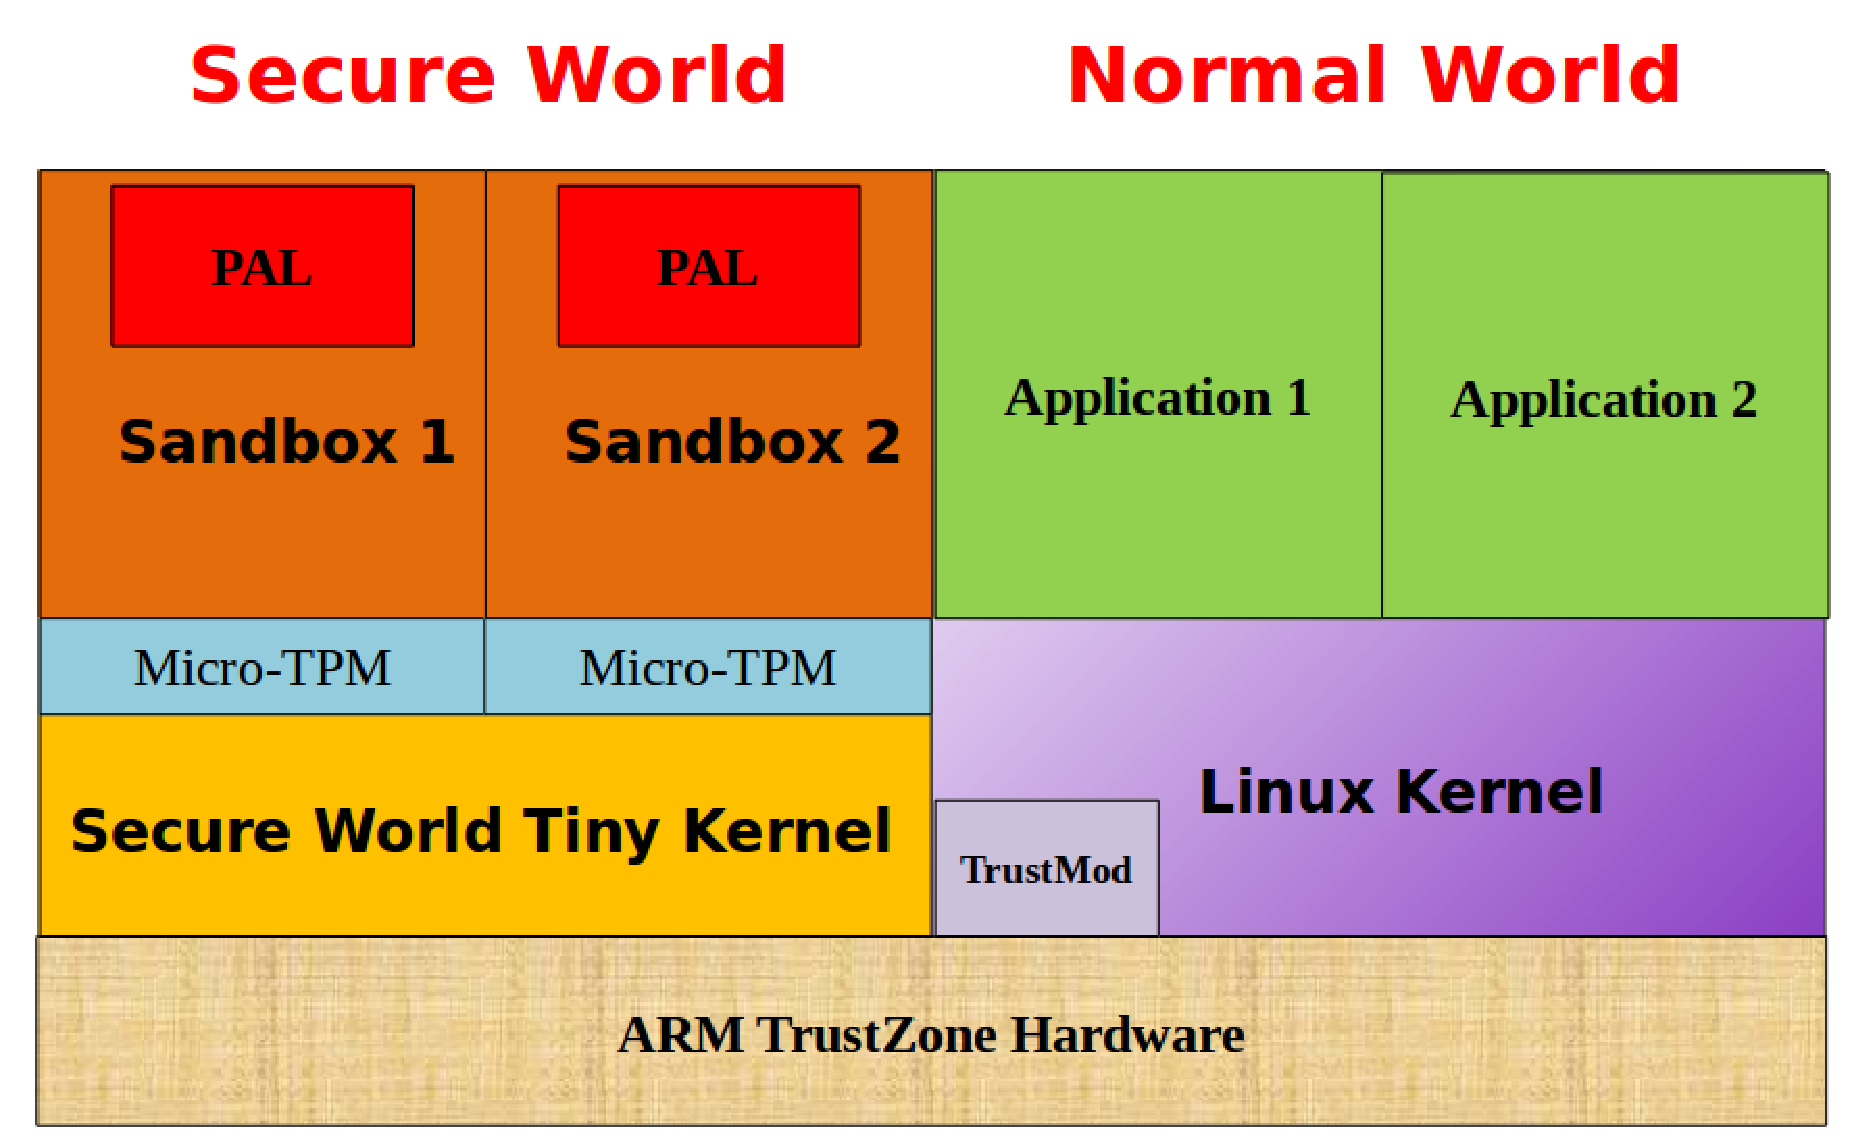
\includegraphics[width=\columnwidth]{figures/future.eps}
\caption{Secure execution of PAL on ARM Architecture}
\label{fig:future}
\end{figure}

Our proposal, as in Figure \ref{fig:future}, leverages the TrustZone, which is
supported by most ARM CPUs, to isolate the secure PAL in the secure world. The
regular OS is running in the normal world while the secure PAL is executed in
the secure world. Unlike virtualization which can create more than one isolated
environments, there is only one secure world with TrustZone. To prevent the
secure PAL of one application from compromising the PAL of another, all PALs
are sandboxed in the secure world. We will use TrustZone to emulate the secure
boot, late launch and TPM operations. As ARM boards usually have limited
resources, the secure world tiny kernel will not be loaded into memory unless
the execution of PAL is registered and triggered. To prevent Iago attack, we
divide the system calls into sensitive calls and non-sensitive calls. All
sensitive calls, which can be used by malicious OS to mount the Iago attack,
will be handled directly by the tiny kernel in secure world. Non-sensitive
calls will be redirected to the untrusted OS in normal world. As the tiny
kernel is only responsible for supporting the Micro-TPM, memory management and
handling sensitive system calls, the TCB is small.
